\documentclass[12pt, a4paper]{article}

% Packages dependencies
\usepackage[brazil]{babel}
\usepackage[top=3cm, bottom=2cm, left=3cm, right=3cm]{geometry}
\usepackage{graphicx}
\usepackage{titlesec}
\usepackage{float}
\usepackage{minted}
\usepackage{xcolor}
\usepackage[labelformat=empty]{caption}
\usepackage{amsmath}
\usepackage{amssymb}
\usepackage{multicol}
\usepackage{indentfirst}
\usepackage{hyperref}
\usepackage{titlesec}
\usepackage{enumitem}
\usepackage[most]{tcolorbox}
\usepackage{cleveref}
\usepackage{fontspec}
\hypersetup{
    colorlinks=true,
    urlcolor=blue,
    linkcolor=blue
}
\setmainfont{ARIAL.TTF}[
  ItalicFont = ARIALI.TTF,
  BoldFont = ARIALBD.TTF,
  BoldItalicFont = ARIALBI.TTF,
  Path = ./fontes/
]
\setmonofont{JetBrains Mono}[
Scale=MatchLowercase,
Ligatures=TeX,
Contextuals=Alternate
]
\newtcolorbox{mybox}[2][]{breakable,sharp corners, skin=enhancedmiddle jigsaw,parbox=false,
boxrule=0mm,leftrule=2mm,boxsep=0mm,arc=0mm,outer arc=0mm,attach title to upper,
after title={.\ }, coltitle=black,colback=gray!10,colframe=black, title={#2},
fonttitle=\bfseries,#1}
\renewcommand*\contentsname{SUMÁRIO}

\graphicspath{{images/}}

%Preamble
\date{\today}

%Variable Student Name
\newcommand\studentName{Matheus de Freitas Weber}
\newcommand\studentTwoName{Gabriel Berwanger Silveira}
\newcommand\studentThreeName{Aluno 3}
\newcommand\studentFourName{Aluno 4}

%Variable Course Name
\newcommand\courseName{Circuitos microprocessados}

%Variable Article Name
\newcommand\titleName{Exercício - Aula 05}

%Variable Article SubName
\newcommand\subTitleName{PWM - Motor CC}

%Variable Teacher Name
\newcommand\teacherName{Jean Schmith}

%Body
\begin{document}

% -- Unisinos title -- %
\begin{center}
	\MakeUppercase{\textbf{Universidade do Vale do Rio dos Sinos (Unisinos)}}

	% -- Course Name -- %
	\MakeUppercase{\textbf{Graduação em Engenharia de controle e automação}} \\[16ex]


	% -- Student Name -- %
	\MakeUppercase{\textbf{\studentName}}
	\\
	\MakeUppercase{\textbf{\studentTwoName}}
	\\[16ex]

	% -- Work Title -- %
	\MakeUppercase{\textbf{\titleName}}

	\textbf{\subTitleName}

	\vfill

	\textbf{São Leopoldo}

	\textbf{2025}

	\thispagestyle{empty}
\end{center}
\newpage

% -- Capa -- %
\begin{center}
	% -- Capa -- %
	\vspace*{28ex}
	\MakeUppercase{\studentName}
	\\
	\MakeUppercase{\studentTwoName}
	\vspace*{16ex}

	\MakeUppercase{\textbf{\titleName}}

	\textbf{\subTitleName}

	\vspace*{8ex}

	% -- Description of the work -- %
	\hfill\begin{minipage}{0.5\linewidth}
		Trabalho apresentado para a matéria {\courseName} pelo Curso de Engenharia de Controle e Automação e Engenharia da Computação da Universidade do Vale do Sinos (UNISINOS), ministrada pelo Prof.\teacherName.
	\end{minipage}
	\vfill

	\textbf{São Leopoldo}

	\textbf{2025}

\end{center}
\thispagestyle{empty}
\setcounter{page}{1}

\newpage
% -- Summary -- %
\begin{center}
	\tableofcontents
\end{center}
\thispagestyle{empty}

\newpage
% -- Introduction -- %
\section{Introdução}
O objetivo deste exercício é utilizar a técnica de PWM (Pulse Width Modulation) para controlar a velocidade de um motor de corrente contínua (CC) utilizando um Arduino Uno. Através da variação do ciclo de trabalho do sinal PWM, é possível ajustar a potência fornecida ao motor, permitindo o controle preciso da sua velocidade. Este método é amplamente utilizado em aplicações de controle de motores devido à sua eficiência e simplicidade.


\newpage
% -- Teorical foundation -- %

\newpage
\section{Metodologia}
\subsection{Materiais Utilizados}
\begin{itemize}
	\item 1x Arduino Uno
	\item 1x Motor de corrente contínua (CC)
	\item Fios de conexão
	\item Ponte H (L298N ou similar)
\end{itemize}

\subsection{Diagrama de Conexões}
\begin{figure}[H]
	\centering
	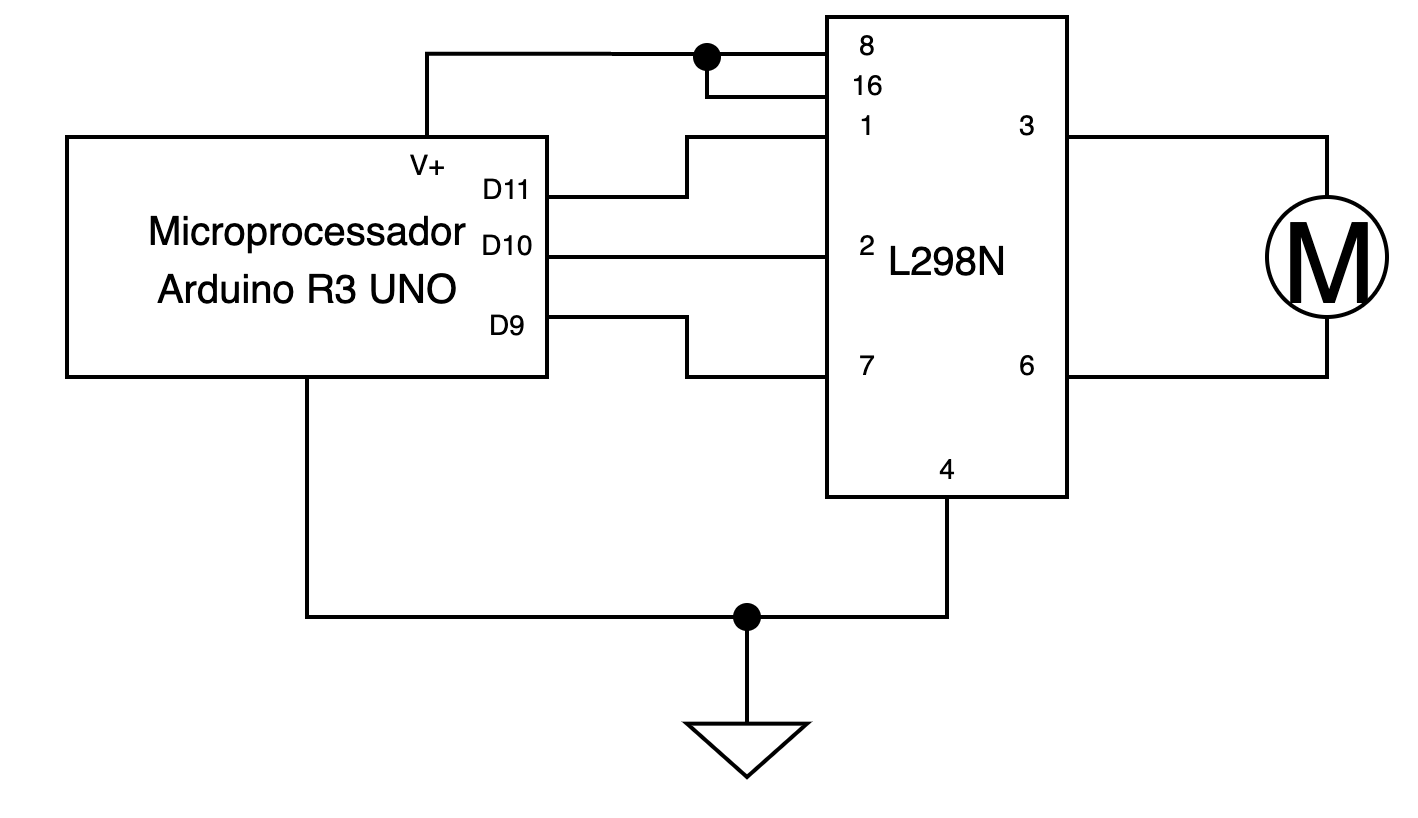
\includegraphics[width=0.8\textwidth]{./images/diagrama_aula05.png}
	\caption{Diagrama de conexões.}
	\label{fig:montagem_protoboard}
\end{figure}
\begin{figure}[H]
	\centering
	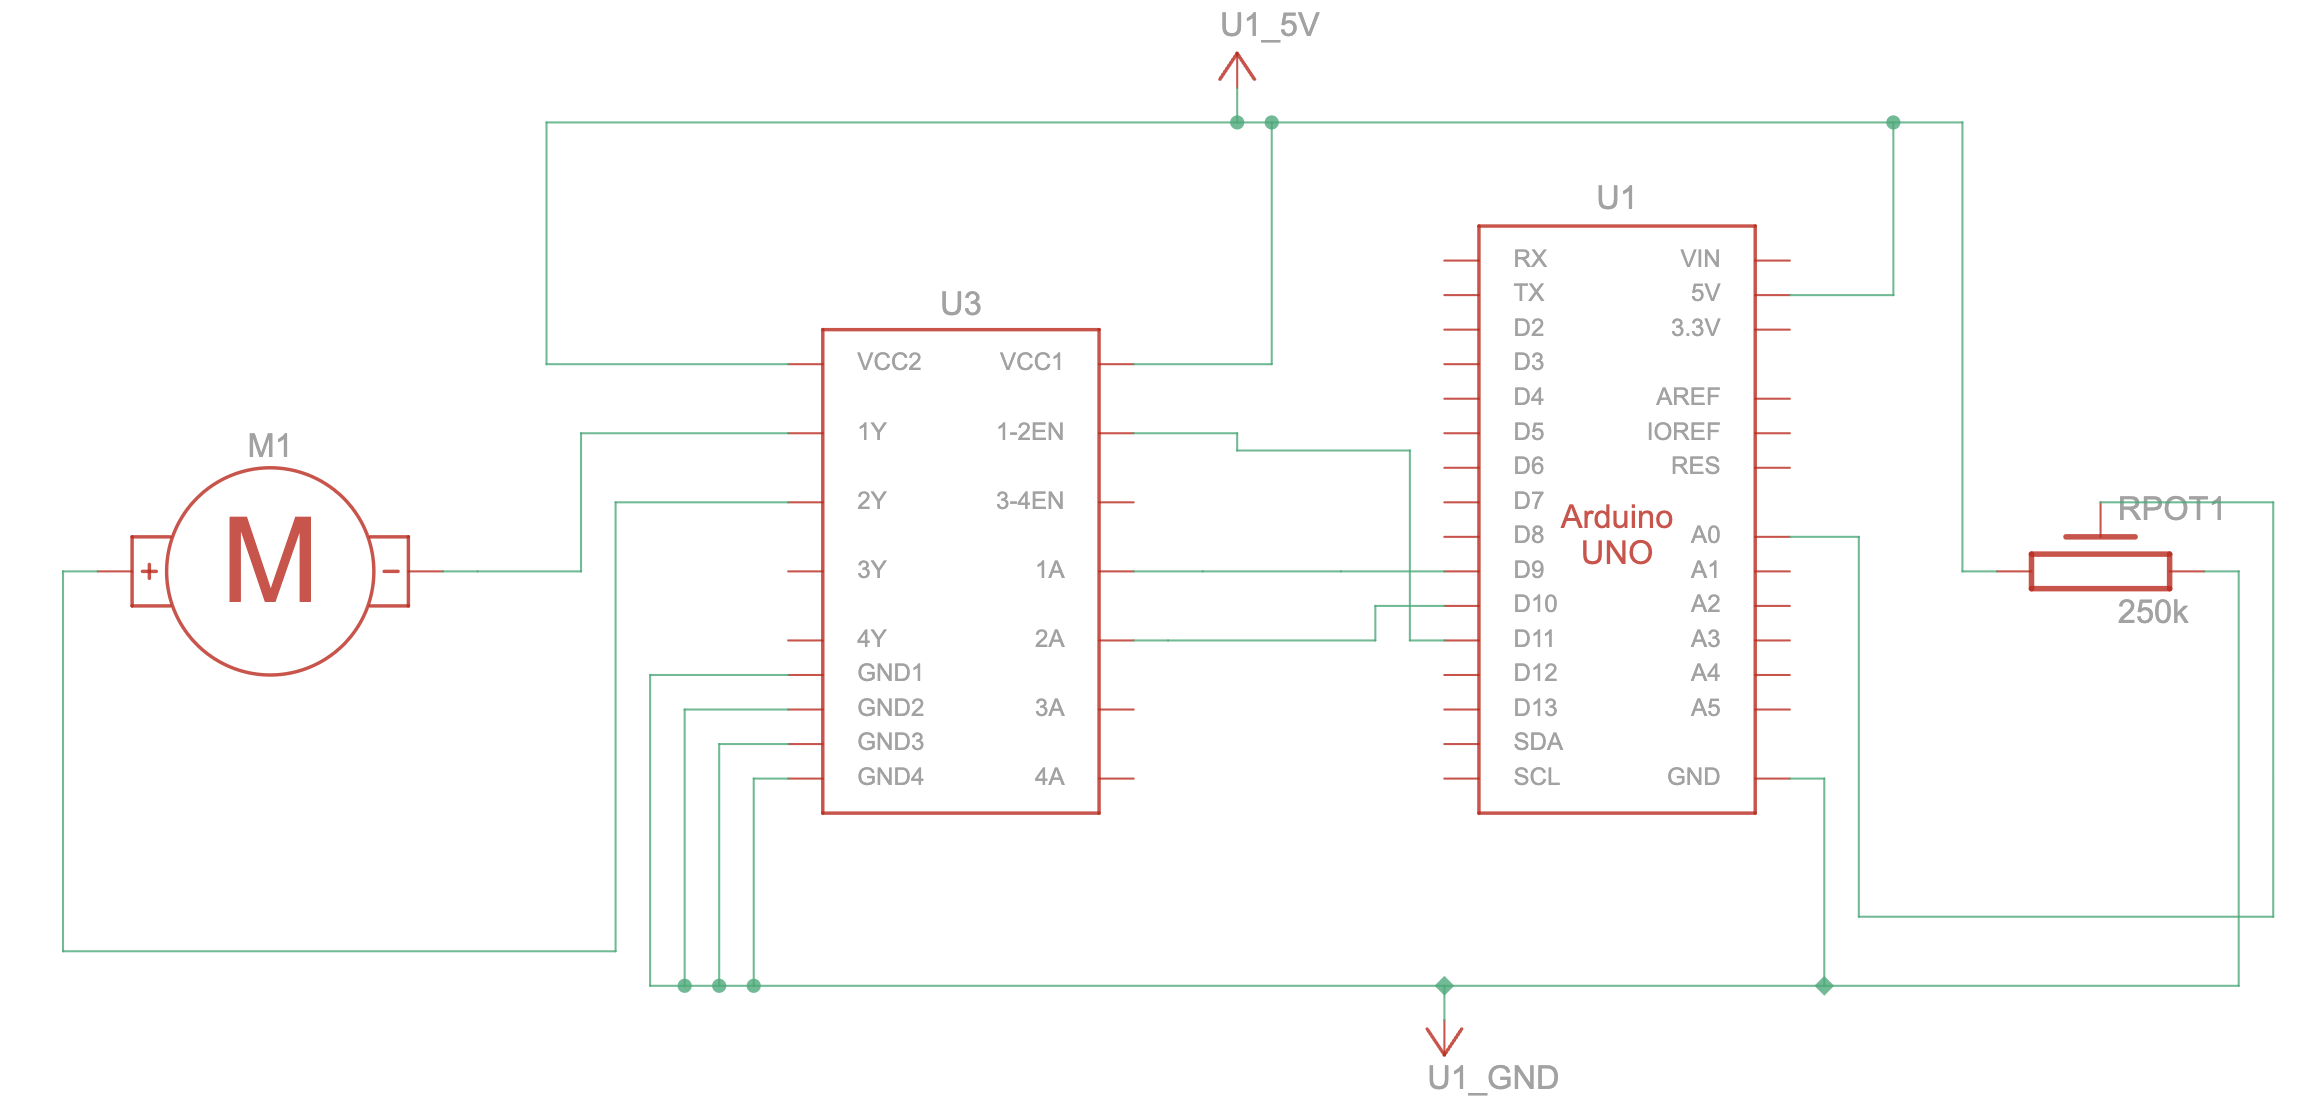
\includegraphics[width=0.8\textwidth]{./images/diagrama_tinkercad_aula05.png}
	\caption{Montagem no TinkerCAD.}
	\label{fig:montagem_protoboard}
\end{figure}

\subsection{Fluxograma}
\begin{figure}[H]
	\centering
	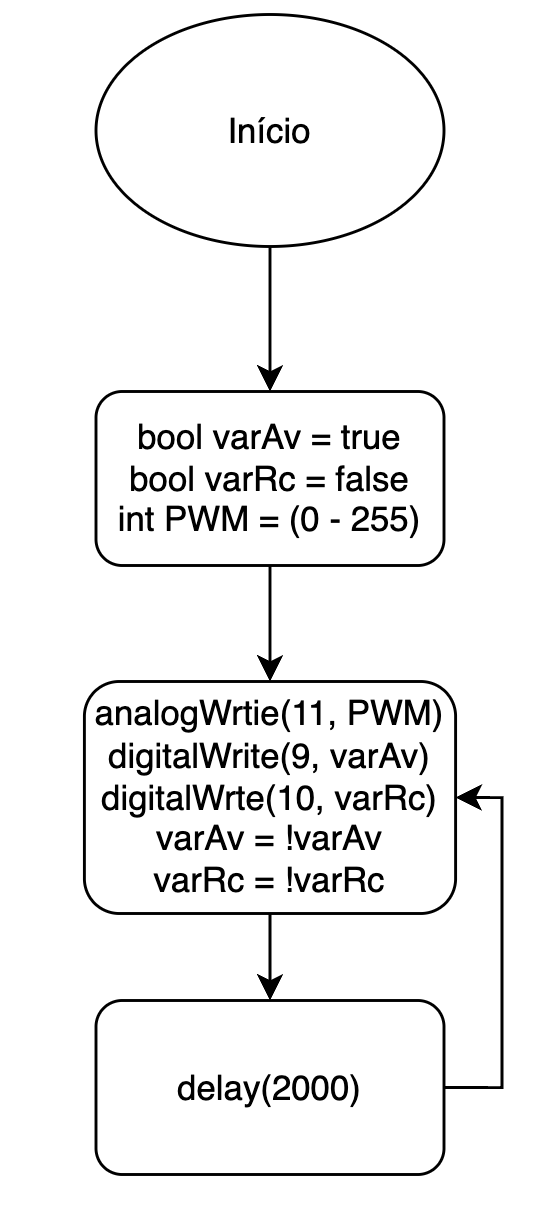
\includegraphics[width=0.6\textwidth]{fluxograma_trabalho_04.png}
	\caption{Fluxograma do controle do motor CC.}
	\label{fig:fluxograma_aula05}
\end{figure}

\subsection{Código Fonte}

\begin{mybox}[label={lst:codigo_servidor},title={Código}]{}
	\inputminted[fontsize=\footnotesize,breaklines,linenos]{cpp}{./arduino/main.ino}
\end{mybox}
\newpage
\section{Resultados}
Com essa montagem foi possível controlar a velocidade do motor CC através do sinal PWM gerado pelo Arduino. Ao variar o ciclo de trabalho do sinal PWM, observou-se uma mudança na velocidade do motor, confirmando a eficácia da técnica de modulação por largura de pulso para controle de motores.

\begin{figure}[H]
	\centering
	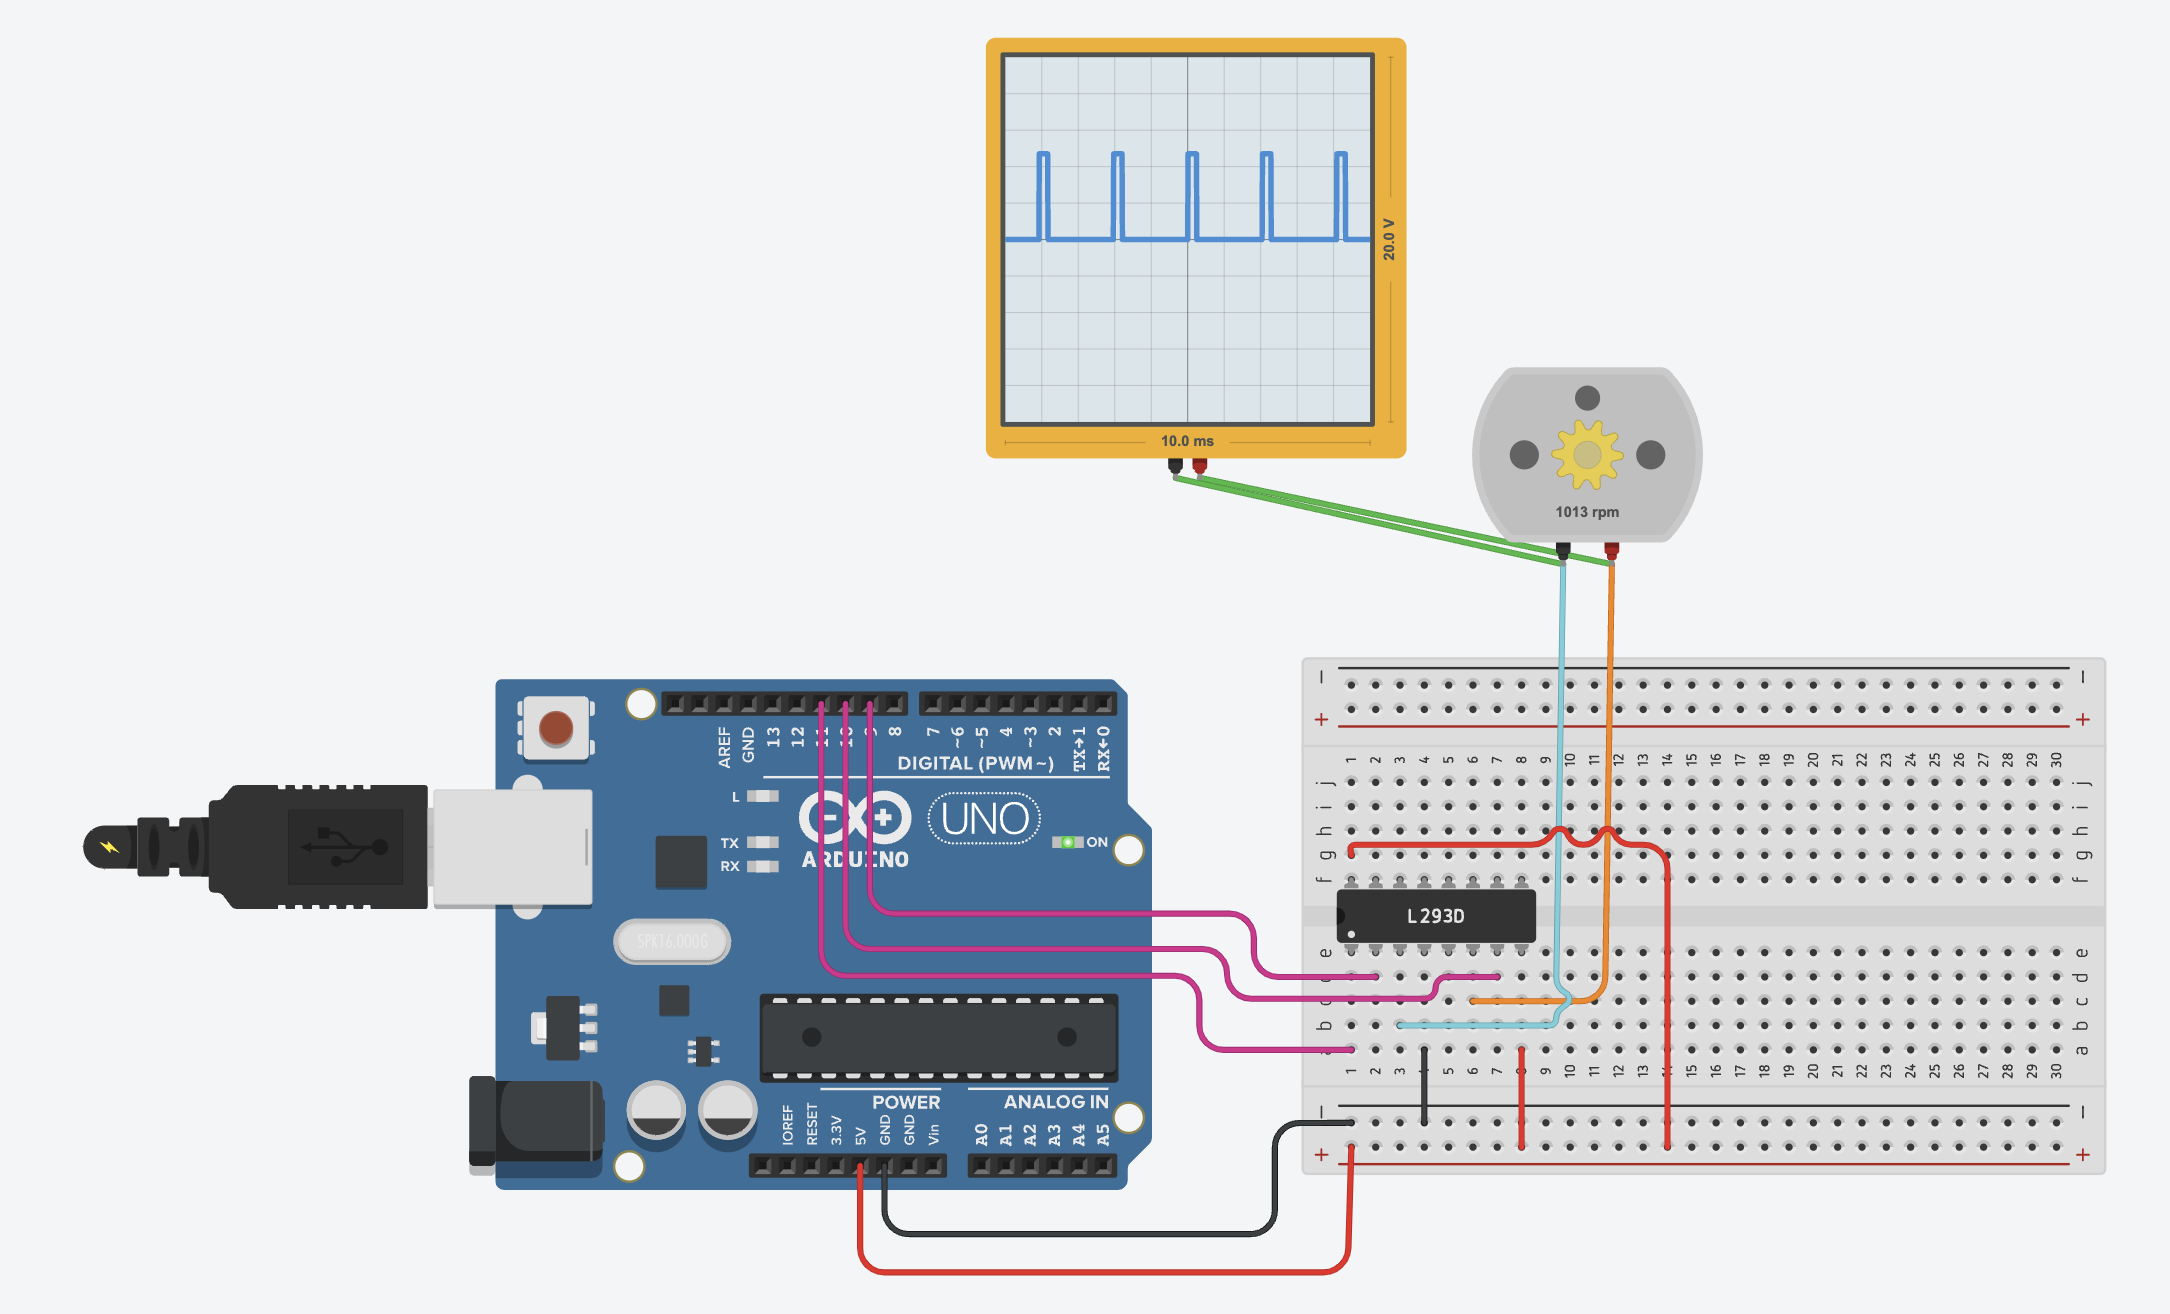
\includegraphics[width=0.8\textwidth]{./images/montagem_tinkercad_aula05.png}
	\caption{Resultado da leitura e controle do motor CC.}
	\label{fig:resultado_leitura}
\end{figure}

\newpage
% -- Conclusion -- %
\begin{center}
	\section{Conclusão}
\end{center}
Através deste exercício, foi possível compreender a aplicação prática da técnica de PWM para o controle de motores de corrente contínua utilizando um Arduino. A variação do ciclo de trabalho do sinal PWM mostrou-se eficaz na regulação da velocidade do motor, demonstrando a importância dessa técnica em sistemas de controle. Além disso, a utilização do Arduino facilitou a implementação e o teste do circuito, tornando o processo mais acessível para estudantes e entusiastas da eletrônica e automação.

\rule{\textwidth}{0.4pt}
\subsubsection{Link do TinkerCAD}
\url{https://www.tinkercad.com/things/1L6fpXbc73m/editel?returnTo=%2Fdashboard&sharecode=wDwXt3oJ5AQZRMxl7saFi12AiarmNFKWnacPJ02lm2M}
\end{document}
